\chapter{\textit{DOWNLOAD} DATA OSM}

QGIS walaupun tergolong dalam perangkat lunak terbuka dan gratis, namun menyediakan fasilitas bukan hanya sebagai editor data spasial, tetapi mampu memberikan beberapa fasilitas analisis, baik terhadap data spasial, maupun data atribut.

Pada Bab ini akan dibahas bagaimana cara memperoleh data spasial dalam format vektor dari \textit{Open Street Map} menggunakan \textit{Tools} yang ada pada QGIS yang mungkin dapat dijadikan salah satu sumber data dalam analisa.

Untuk melakukan pengambilan data dari OSM, QGIS memerlukan 2 (dua) \textit{plugins}, adapun tahapan-tahapan yang dapat dilakukan sebagai berikut :

\begin{enumerate}[1.]
  \item Meng\textit{install plugin} \textbf{OSMDownloader} dan \textbf{OpenLayers} melalui menu \texttt{Plugins > Manage and Install Plugins...} seperti pada gambar \ref{fig:managepluginsmenu}.
  
  \begin{figure}[H]
    \centering
    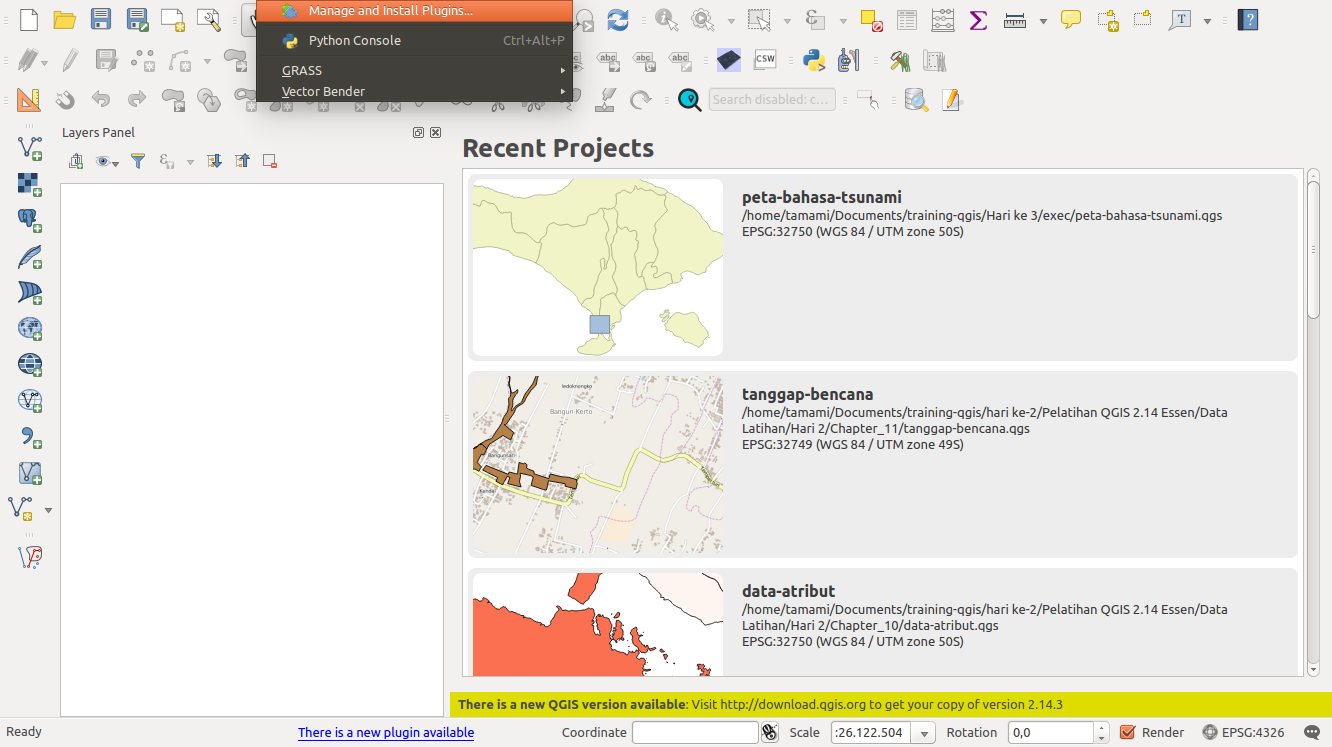
\includegraphics[width=1\textwidth]{./resources/001-manage-plugins-menu}
    \caption{Menu \textit{Manage Plugins}}
    \label{fig:managepluginsmenu}
  \end{figure}
  
  \item Kemudian ketik kata kunci \texttt{OSM} di bagian \textit{search} pada kotak dialog dibagian atas dan pilih komponen seperti pada gambar \ref{fig:osminstallwin}. Komponen \textit{OpenLayers Plugin} digunakan untuk menampilkan \textit{basemap}, sedangkan komponen \textit{OSMDownloader} adalah perangkat yang digunakan untuk mengambil data dari OSM baik yang berbentuk spasial (vektor) maupun data atribut yang tersimpan disana.
  
  \begin{figure}[H]
    \centering
    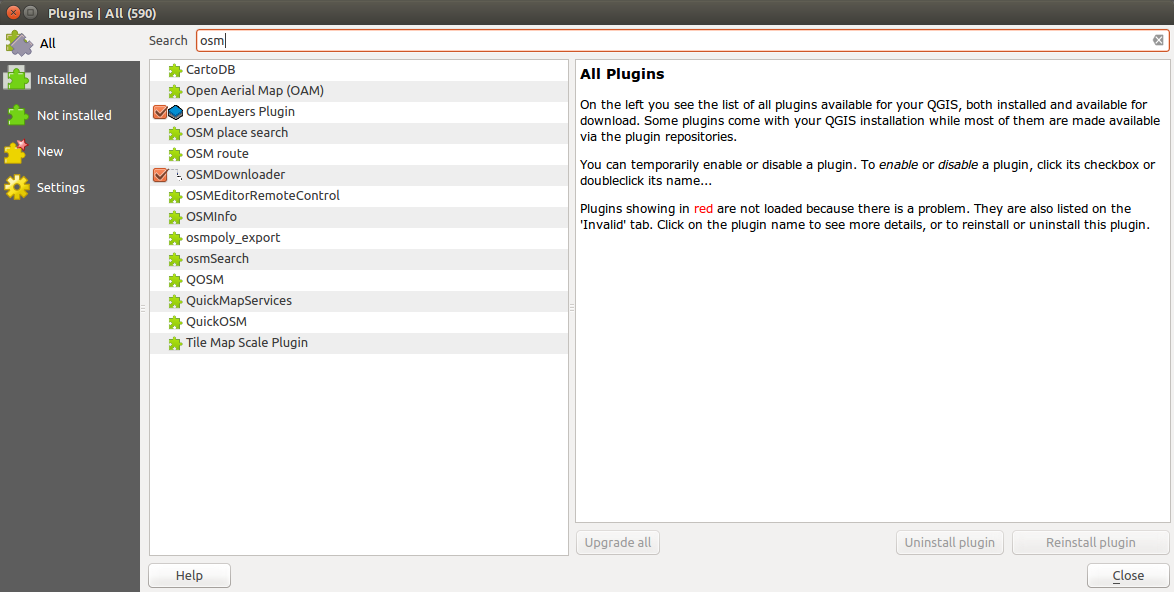
\includegraphics[width=1\textwidth]{./resources/002-osm-install-win}
    \caption{Jendela \textit{Manage Plugins}}
    \label{fig:osminstallwin}
  \end{figure}
  
  \item Setelah kedua komponen seperti pada gambar \ref{fig:osminstallwin} terpilih, maka klik tombol \textit{Install Plugin} di bagian kanan bawah untuk memasangkan peralatan OSM.
  
  \item \textit{Plugin} \textbf{OpenLayers} memperbolehkan untuk mengakses \textit{basemap} dari berbagai provider yang disediakan QGIS. Contohnya adalah, membuka OSM \textit{basemap} dengan cara memilih menu \texttt{Web > OpenLayers Plugin > OpenStreetMap > OpenStreetMap} seperti pada gambar \ref{fig:osmmenu}. Sebagai catatan, untuk menjalankan \textit{OpenLayers} diperlukan akses internet.
  
  \begin{figure}[H]
    \centering
    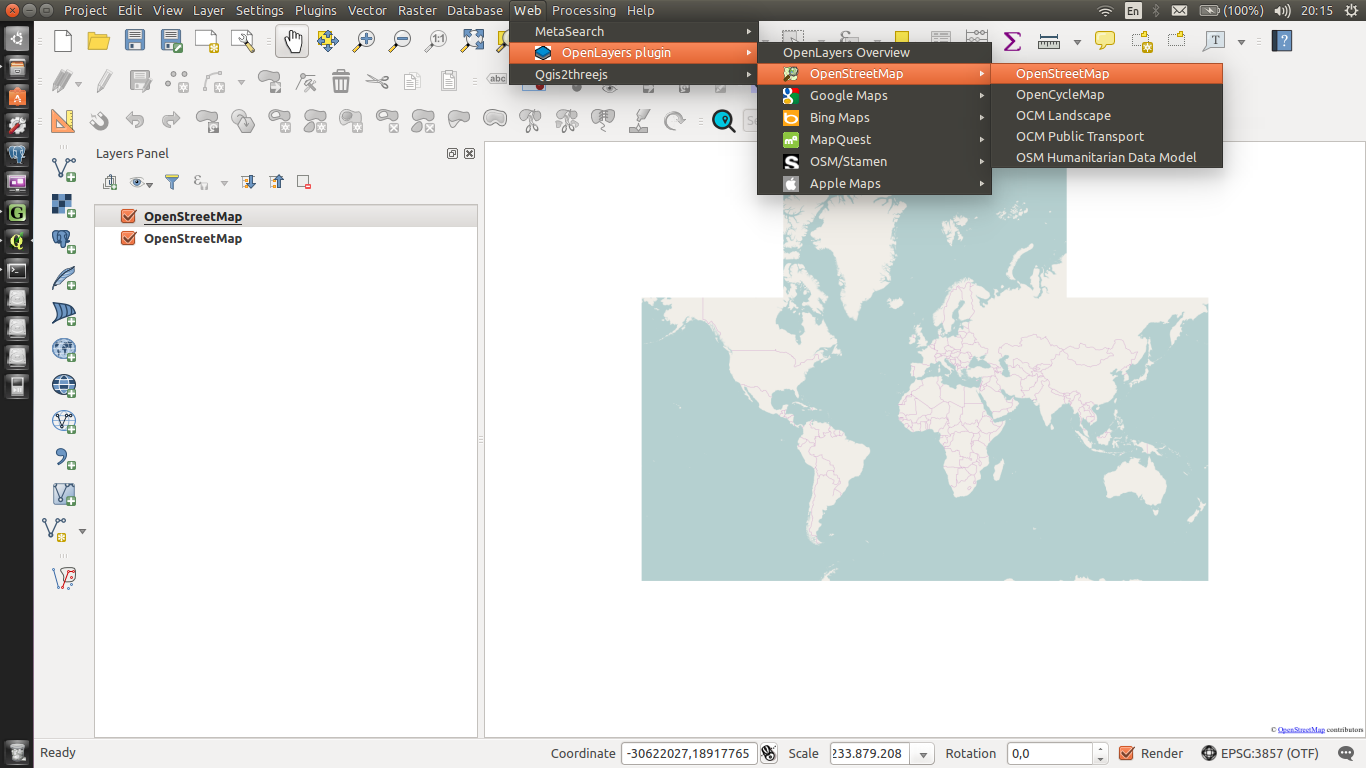
\includegraphics[width=1\textwidth]{./resources/003-osm-plugin-menu}
    \caption{Menu \textit{Open Layers}}
    \label{fig:osmmenu}
  \end{figure}
  
  \item Dari kondisi \textit{basemap} yang sudah diperbesar dan difokuskan untuk wilayah tertentu, maka dapat diambil data spasial dan atribut untuk wilayah tertentu di OSM, gunakan menu \texttt{Vector > OpenStreetMap > Download Data} seperti pada gambar \ref{fig:downloadosmmenu}
  
  \begin{figure}[H]
    \centering
    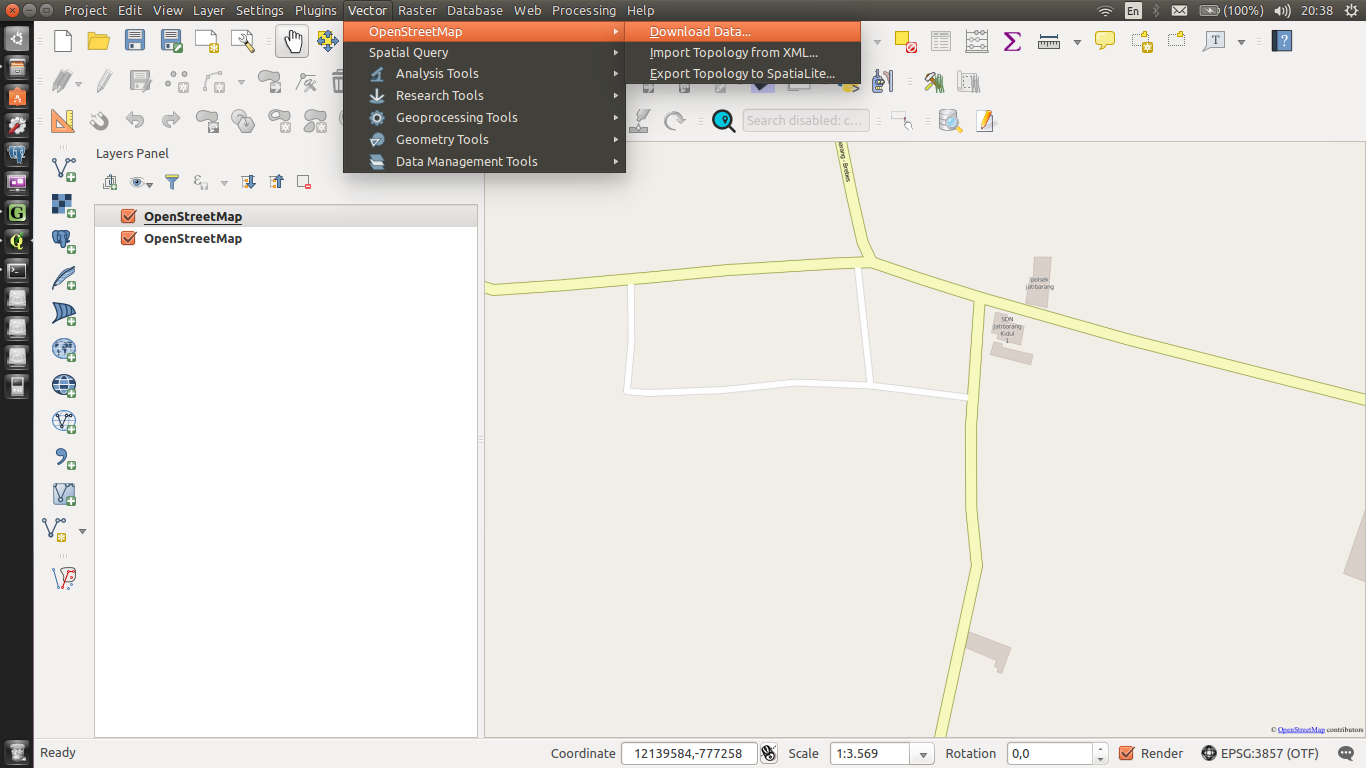
\includegraphics[width=1\textwidth]{./resources/004-download-osm-menu}
    \caption{Menu \textit{Download} OSM Data}
    \label{fig:downloadosmmenu}
  \end{figure}
\end{enumerate}